% interactcadsample.tex
% v1.03 - April 2017

\documentclass[]{interact}

\usepackage{epstopdf}% To incorporate .eps illustrations using PDFLaTeX, etc.
\usepackage{subfigure}% Support for small, `sub' figures and tables
%\usepackage[nolists,tablesfirst]{endfloat}% To `separate' figures and tables from text if required
% \usepackage[utf8]{inputenc}

\usepackage{natbib}% Citation support using natbib.sty
\bibpunct[, ]{(}{)}{;}{a}{}{,}% Citation support using natbib.sty
\renewcommand\bibfont{\fontsize{10}{12}\selectfont}% Bibliography support using natbib.sty

\theoremstyle{plain}% Theorem-like structures provided by amsthm.sty
\newtheorem{theorem}{Theorem}[section]
\newtheorem{lemma}[theorem]{Lemma}
\newtheorem{corollary}[theorem]{Corollary}
\newtheorem{proposition}[theorem]{Proposition}

\theoremstyle{definition}
\newtheorem{definition}[theorem]{Definition}
\newtheorem{example}[theorem]{Example}

\theoremstyle{remark}
\newtheorem{remark}{Remark}
\newtheorem{notation}{Notation}

% see https://stackoverflow.com/a/47122900
  \usepackage{color}
  \usepackage{fancyvrb}
  \newcommand{\VerbBar}{|}
  \newcommand{\VERB}{\Verb[commandchars=\\\{\}]}
  \DefineVerbatimEnvironment{Highlighting}{Verbatim}{commandchars=\\\{\}}
  % Add ',fontsize=\small' for more characters per line
  \usepackage{framed}
  \definecolor{shadecolor}{RGB}{248,248,248}
  \newenvironment{Shaded}{\begin{snugshade}}{\end{snugshade}}
  \newcommand{\AlertTok}[1]{\textcolor[rgb]{0.94,0.16,0.16}{#1}}
  \newcommand{\AnnotationTok}[1]{\textcolor[rgb]{0.56,0.35,0.01}{\textbf{\textit{#1}}}}
  \newcommand{\AttributeTok}[1]{\textcolor[rgb]{0.77,0.63,0.00}{#1}}
  \newcommand{\BaseNTok}[1]{\textcolor[rgb]{0.00,0.00,0.81}{#1}}
  \newcommand{\BuiltInTok}[1]{#1}
  \newcommand{\CharTok}[1]{\textcolor[rgb]{0.31,0.60,0.02}{#1}}
  \newcommand{\CommentTok}[1]{\textcolor[rgb]{0.56,0.35,0.01}{\textit{#1}}}
  \newcommand{\CommentVarTok}[1]{\textcolor[rgb]{0.56,0.35,0.01}{\textbf{\textit{#1}}}}
  \newcommand{\ConstantTok}[1]{\textcolor[rgb]{0.00,0.00,0.00}{#1}}
  \newcommand{\ControlFlowTok}[1]{\textcolor[rgb]{0.13,0.29,0.53}{\textbf{#1}}}
  \newcommand{\DataTypeTok}[1]{\textcolor[rgb]{0.13,0.29,0.53}{#1}}
  \newcommand{\DecValTok}[1]{\textcolor[rgb]{0.00,0.00,0.81}{#1}}
  \newcommand{\DocumentationTok}[1]{\textcolor[rgb]{0.56,0.35,0.01}{\textbf{\textit{#1}}}}
  \newcommand{\ErrorTok}[1]{\textcolor[rgb]{0.64,0.00,0.00}{\textbf{#1}}}
  \newcommand{\ExtensionTok}[1]{#1}
  \newcommand{\FloatTok}[1]{\textcolor[rgb]{0.00,0.00,0.81}{#1}}
  \newcommand{\FunctionTok}[1]{\textcolor[rgb]{0.00,0.00,0.00}{#1}}
  \newcommand{\ImportTok}[1]{#1}
  \newcommand{\InformationTok}[1]{\textcolor[rgb]{0.56,0.35,0.01}{\textbf{\textit{#1}}}}
  \newcommand{\KeywordTok}[1]{\textcolor[rgb]{0.13,0.29,0.53}{\textbf{#1}}}
  \newcommand{\NormalTok}[1]{#1}
  \newcommand{\OperatorTok}[1]{\textcolor[rgb]{0.81,0.36,0.00}{\textbf{#1}}}
  \newcommand{\OtherTok}[1]{\textcolor[rgb]{0.56,0.35,0.01}{#1}}
  \newcommand{\PreprocessorTok}[1]{\textcolor[rgb]{0.56,0.35,0.01}{\textit{#1}}}
  \newcommand{\RegionMarkerTok}[1]{#1}
  \newcommand{\SpecialCharTok}[1]{\textcolor[rgb]{0.00,0.00,0.00}{#1}}
  \newcommand{\SpecialStringTok}[1]{\textcolor[rgb]{0.31,0.60,0.02}{#1}}
  \newcommand{\StringTok}[1]{\textcolor[rgb]{0.31,0.60,0.02}{#1}}
  \newcommand{\VariableTok}[1]{\textcolor[rgb]{0.00,0.00,0.00}{#1}}
  \newcommand{\VerbatimStringTok}[1]{\textcolor[rgb]{0.31,0.60,0.02}{#1}}
  \newcommand{\WarningTok}[1]{\textcolor[rgb]{0.56,0.35,0.01}{\textbf{\textit{#1}}}}
    
  % Pandoc citation processing

\usepackage{hyperref}
\usepackage[utf8]{inputenc}
\usepackage{float}
\floatplacement{figure}{H}
\def\tightlist{}
\newcommand{\beginsupplement}{\setcounter{table}{0}  \renewcommand{\thetable}{S\arabic{table}} \setcounter{figure}{0} \renewcommand{\thefigure}{S\arabic{figure}}}
\usepackage{booktabs}
\usepackage{longtable}
\usepackage{array}
\usepackage{multirow}
\usepackage{wrapfig}
\usepackage{float}
\usepackage{colortbl}
\usepackage{pdflscape}
\usepackage{tabu}
\usepackage{threeparttable}
\usepackage{threeparttablex}
\usepackage[normalem]{ulem}
\usepackage{makecell}
\usepackage{xcolor}
\usepackage{multicol}
\usepackage{hhline}
\usepackage{hyperref}

\begin{document}

\articletype{Technical Report}

\title{DRAFT: Evaluation of Algal bloom potential for the Caloosahatchee
River Estuary}


\author{\name{Paul Julian$^{1,2}$}
\affil{$^{1}$Sanibel-Captiva Conservation Foundation, PO Box 839,
Sanibel, FL 33957\\ $^{2}$Conservancy of Southwest Florida, 1495 Smith
Preserve Way, Naples, FL 34102}
}

\thanks{CONTACT Paul
Julian. Email: \href{mailto:pjulian@sccf.org}{\nolinkurl{pjulian@sccf.org}}}

\maketitle



\begin{github}
\url{https://github.com/SwampThingPaul/LOSOM_AlgalBloom/}
\end{github}

\begin{DOI}
\url{https://doi.org/10.5281/zenodo.4876353}
\end{DOI}

\hypertarget{objective}{%
\section{Objective}\label{objective}}

The draft Northern Estuaries Algal Bloom Risk Assessment performance
measure for Lake Okeechobee System Operating Manual (LOSOM) proposes to
evaluate changes in discharges from Lake Okeechobee to the
Caloosahatchee River Estuary (CRE) to assess the risk of algal bloom
development. The premise of this performance measure is that releasing
freshwater with sufficient algal biomass to the estuaries during the
summer (May/June - August) favors freshwater algal blooms in the
estuaries by transport of algal biomass, expansion of the freshwater
habitat suitable for algal growth, and subsidizing available nutrients.
This concept has been demonstrated for the St Lucie Estuary
\citep{phlips_hurricanes_2020} but not for the CRE. Therefore, this
preliminary evaluation will explore the potential for algal bloom
transport from Lake Okeechobee to the CRE and the role of discharges on
algal bloom formation at the CRE headwaters.

\hypertarget{methods}{%
\section{Methods}\label{methods}}

\hypertarget{data-source}{%
\subsection{Data Source}\label{data-source}}

Chlorophyll-a data were retrieved from the South Florida Water
Management District (SFWMD) online database (DBHYDRO;
\url{www.sfwmd.gov/dbhydro}) for sites defined as Lake Okeechobee
western littoral zone as defined by \citet{walker_draft_2020} and S-79
(Table \ref{tab:tab1}) for S-77 and S-79. Only positive discharge values
were considered in this analysis, therefore discharge values reported
less than zero were replaced with zero. Water quality data were screened
based on laboratory qualifier codes, consistent with Florida Department
of Environmental Protection's quality assurance rule
\citep{florida_administrative_code_chapter_2008}. Any datum associated
with a fatal qualifier indicating a potential data quality problem was
removed from the analysis. Additional considerations in the handling of
analytical data were the accuracy and sensitivity of the laboratory
method used. For purposes of data analysis and summary statistics, data
reported as less than the method detection limit (MDL) were assigned
one-half the MDL.

\providecommand{\docline}[3]{\noalign{\global\setlength{\arrayrulewidth}{#1}}\arrayrulecolor[HTML]{#2}\cline{#3}}

\setlength{\tabcolsep}{2pt}

\renewcommand*{\arraystretch}{1.5}

\begin{longtable}[c]{|p{1.21in}|p{1.02in}|p{2.52in}}

\caption{\label{tab:tab1} Monitoring Locations used in this evaluation with regions defined. A map of mointoring locations is presented in Fig \ref{fig:map}.}\\

\hhline{>{\arrayrulecolor[HTML]{666666}\global\arrayrulewidth=2pt}->{\arrayrulecolor[HTML]{666666}\global\arrayrulewidth=2pt}->{\arrayrulecolor[HTML]{666666}\global\arrayrulewidth=2pt}-}

\multicolumn{1}{!{\color[HTML]{000000}\vrule width 0pt}>{\raggedright}p{\dimexpr 1.21in+0\tabcolsep+0\arrayrulewidth}}{\fontsize{11}{11}\selectfont{\textcolor[HTML]{000000}{DataType}}} & \multicolumn{1}{!{\color[HTML]{000000}\vrule width 0pt}>{\raggedright}p{\dimexpr 1.02in+0\tabcolsep+0\arrayrulewidth}}{\fontsize{11}{11}\selectfont{\textcolor[HTML]{000000}{Site}}} & \multicolumn{1}{!{\color[HTML]{000000}\vrule width 0pt}>{\raggedright}p{\dimexpr 2.52in+0\tabcolsep+0\arrayrulewidth}!{\color[HTML]{000000}\vrule width 0pt}}{\fontsize{11}{11}\selectfont{\textcolor[HTML]{000000}{Region}}} \\

\noalign{\global\setlength{\arrayrulewidth}{2pt}}\arrayrulecolor[HTML]{666666}\cline{1-3}

\endfirsthead

\hhline{>{\arrayrulecolor[HTML]{666666}\global\arrayrulewidth=2pt}->{\arrayrulecolor[HTML]{666666}\global\arrayrulewidth=2pt}->{\arrayrulecolor[HTML]{666666}\global\arrayrulewidth=2pt}-}

\multicolumn{1}{!{\color[HTML]{000000}\vrule width 0pt}>{\raggedright}p{\dimexpr 1.21in+0\tabcolsep+0\arrayrulewidth}}{\fontsize{11}{11}\selectfont{\textcolor[HTML]{000000}{DataType}}} & \multicolumn{1}{!{\color[HTML]{000000}\vrule width 0pt}>{\raggedright}p{\dimexpr 1.02in+0\tabcolsep+0\arrayrulewidth}}{\fontsize{11}{11}\selectfont{\textcolor[HTML]{000000}{Site}}} & \multicolumn{1}{!{\color[HTML]{000000}\vrule width 0pt}>{\raggedright}p{\dimexpr 2.52in+0\tabcolsep+0\arrayrulewidth}!{\color[HTML]{000000}\vrule width 0pt}}{\fontsize{11}{11}\selectfont{\textcolor[HTML]{000000}{Region}}} \\

\noalign{\global\setlength{\arrayrulewidth}{2pt}}\arrayrulecolor[HTML]{666666}\cline{1-3}\endhead



\multicolumn{1}{!{\color[HTML]{000000}\vrule width 0pt}>{\raggedright}p{\dimexpr 1.21in+0\tabcolsep+0\arrayrulewidth}}{} & \multicolumn{1}{!{\color[HTML]{000000}\vrule width 0pt}>{\raggedright}p{\dimexpr 1.02in+0\tabcolsep+0\arrayrulewidth}}{\fontsize{11}{11}\selectfont{\textcolor[HTML]{000000}{S79}}} & \multicolumn{1}{!{\color[HTML]{000000}\vrule width 0pt}>{\raggedright}p{\dimexpr 2.52in+0\tabcolsep+0\arrayrulewidth}!{\color[HTML]{000000}\vrule width 0pt}}{\fontsize{11}{11}\selectfont{\textcolor[HTML]{000000}{S-79 (CRE)}}} \\





\multicolumn{1}{!{\color[HTML]{000000}\vrule width 0pt}>{\raggedright}p{\dimexpr 1.21in+0\tabcolsep+0\arrayrulewidth}}{} & \multicolumn{1}{!{\color[HTML]{000000}\vrule width 0pt}>{\raggedright}p{\dimexpr 1.02in+0\tabcolsep+0\arrayrulewidth}}{\fontsize{11}{11}\selectfont{\textcolor[HTML]{000000}{CES01}}} & \multicolumn{1}{!{\color[HTML]{000000}\vrule width 0pt}>{\raggedright}p{\dimexpr 2.52in+0\tabcolsep+0\arrayrulewidth}!{\color[HTML]{000000}\vrule width 0pt}}{\fontsize{11}{11}\selectfont{\textcolor[HTML]{000000}{S-79 (CRE)}}} \\





\multicolumn{1}{!{\color[HTML]{000000}\vrule width 0pt}>{\raggedright}p{\dimexpr 1.21in+0\tabcolsep+0\arrayrulewidth}}{} & \multicolumn{1}{!{\color[HTML]{000000}\vrule width 0pt}>{\raggedright}p{\dimexpr 1.02in+0\tabcolsep+0\arrayrulewidth}}{\fontsize{11}{11}\selectfont{\textcolor[HTML]{000000}{S77}}} & \multicolumn{1}{!{\color[HTML]{000000}\vrule width 0pt}>{\raggedright}p{\dimexpr 2.52in+0\tabcolsep+0\arrayrulewidth}!{\color[HTML]{000000}\vrule width 0pt}}{\fontsize{11}{11}\selectfont{\textcolor[HTML]{000000}{Littoral West (Lake Okeechobee)}}} \\





\multicolumn{1}{!{\color[HTML]{000000}\vrule width 0pt}>{\raggedright}p{\dimexpr 1.21in+0\tabcolsep+0\arrayrulewidth}}{} & \multicolumn{1}{!{\color[HTML]{000000}\vrule width 0pt}>{\raggedright}p{\dimexpr 1.02in+0\tabcolsep+0\arrayrulewidth}}{\fontsize{11}{11}\selectfont{\textcolor[HTML]{000000}{PALMOUT}}} & \multicolumn{1}{!{\color[HTML]{000000}\vrule width 0pt}>{\raggedright}p{\dimexpr 2.52in+0\tabcolsep+0\arrayrulewidth}!{\color[HTML]{000000}\vrule width 0pt}}{\fontsize{11}{11}\selectfont{\textcolor[HTML]{000000}{Littoral West (Lake Okeechobee)}}} \\





\multicolumn{1}{!{\color[HTML]{000000}\vrule width 0pt}>{\raggedright}p{\dimexpr 1.21in+0\tabcolsep+0\arrayrulewidth}}{} & \multicolumn{1}{!{\color[HTML]{000000}\vrule width 0pt}>{\raggedright}p{\dimexpr 1.02in+0\tabcolsep+0\arrayrulewidth}}{\fontsize{11}{11}\selectfont{\textcolor[HTML]{000000}{PLN2OUT}}} & \multicolumn{1}{!{\color[HTML]{000000}\vrule width 0pt}>{\raggedright}p{\dimexpr 2.52in+0\tabcolsep+0\arrayrulewidth}!{\color[HTML]{000000}\vrule width 0pt}}{\fontsize{11}{11}\selectfont{\textcolor[HTML]{000000}{Littoral West (Lake Okeechobee)}}} \\





\multicolumn{1}{!{\color[HTML]{000000}\vrule width 0pt}>{\raggedright}p{\dimexpr 1.21in+0\tabcolsep+0\arrayrulewidth}}{\multirow[t]{-6}{*}{\fontsize{11}{11}\selectfont{\textcolor[HTML]{000000}{Water Quality}}}} & \multicolumn{1}{!{\color[HTML]{000000}\vrule width 0pt}>{\raggedright}p{\dimexpr 1.02in+0\tabcolsep+0\arrayrulewidth}}{\fontsize{11}{11}\selectfont{\textcolor[HTML]{000000}{TREEOUT}}} & \multicolumn{1}{!{\color[HTML]{000000}\vrule width 0pt}>{\raggedright}p{\dimexpr 2.52in+0\tabcolsep+0\arrayrulewidth}!{\color[HTML]{000000}\vrule width 0pt}}{\fontsize{11}{11}\selectfont{\textcolor[HTML]{000000}{Littoral West (Lake Okeechobee)}}} \\





\multicolumn{1}{!{\color[HTML]{000000}\vrule width 0pt}>{\raggedright}p{\dimexpr 1.21in+0\tabcolsep+0\arrayrulewidth}}{} & \multicolumn{1}{!{\color[HTML]{000000}\vrule width 0pt}>{\raggedright}p{\dimexpr 1.02in+0\tabcolsep+0\arrayrulewidth}}{\fontsize{11}{11}\selectfont{\textcolor[HTML]{000000}{S77}}} & \multicolumn{1}{!{\color[HTML]{000000}\vrule width 0pt}>{\raggedright}p{\dimexpr 2.52in+0\tabcolsep+0\arrayrulewidth}!{\color[HTML]{000000}\vrule width 0pt}}{\fontsize{11}{11}\selectfont{\textcolor[HTML]{000000}{From Lake (DBKEY:15635)}}} \\





\multicolumn{1}{!{\color[HTML]{000000}\vrule width 0pt}>{\raggedright}p{\dimexpr 1.21in+0\tabcolsep+0\arrayrulewidth}}{\multirow[t]{-2}{*}{\fontsize{11}{11}\selectfont{\textcolor[HTML]{000000}{Discharge}}}} & \multicolumn{1}{!{\color[HTML]{000000}\vrule width 0pt}>{\raggedright}p{\dimexpr 1.02in+0\tabcolsep+0\arrayrulewidth}}{\fontsize{11}{11}\selectfont{\textcolor[HTML]{000000}{S79}}} & \multicolumn{1}{!{\color[HTML]{000000}\vrule width 0pt}>{\raggedright}p{\dimexpr 2.52in+0\tabcolsep+0\arrayrulewidth}!{\color[HTML]{000000}\vrule width 0pt}}{\fontsize{11}{11}\selectfont{\textcolor[HTML]{000000}{To Estuary (DBKEY: 00865)}}} \\

\noalign{\global\setlength{\arrayrulewidth}{2pt}}\arrayrulecolor[HTML]{666666}\cline{1-3}

\end{longtable}

\hypertarget{data-analysis}{%
\subsection{Data Analysis}\label{data-analysis}}

Daily discharge data were aggregated by month for each discharge
location. Basin discharge was estimated by taking the difference from
S77 and S79. If the difference between the estuary discharge (S79) and
lake (S77) were less than zero then basin discharge was set to zero.
Lake discharges to the estuary were determined based on the relative
discharge volumes of S77 and S79. If S77 discharges were greater than
S79 for any given month it was assumed that the discharge volume at S79
was from the lake (i.e.~no basin flow), otherwise, the observed
discharge volumes for S77 were characterized as lake water. Monthly
discharge volumes were compared between high (June -- August) and low
(September -- May) algal bloom risk periods for S77 and S79 using the
Kruskal-Wallis rank-sum test. The algal bloom risk periods were based on
analyses by Walker (2020), where generally chlorophyll-a concentrations
and therefore algal bloom potential are greatest during May through
August period. The period was adjusted for the CRE as May is typically
the driest month and discharges during this period do not reflect a high
risk of algal transport to the estuary. Monthly mean chlorophyll-a data
were estimated for each region (i.e.~CRE and Littoral West), for Lake
Okeechobee Littoral West all sites were average together for any given
month. Monthly mean chlorophyll-a concentrations were compared between
regions using Kruskal-Wallis rank-sum test. Cross-correlation function
estimation was used to evaluate potential lagged correlations between
Lake Okeechobee (littoral west) and S-79 (CRE) chlorophyll
concentrations where CRE chlorophyll values remained fixed and Lake
Okeechobee chlorophyll values were lagged. Logistic regression was used
to evaluate the potential of bloom formation relative to Lake
discharges. Potential algal blooms at S79 were identified if monthly
mean chlorophyll-a concentrations were greater than 20 \(\mu\)g
L\(^{-1}\).

All plots were generated in base R and all tables were formatted using
``flextable'' R-package \citep{gohel_flextable_2021}. All statistical
operations were performed using R (Ver 4.0.4, R Foundation for
Statistical Computing, Vienna Austria). Unless otherwise stated, all
statistical operations were performed using the base R library. The
critical level of significance was set at \(\alpha\) = 0.05. All
\texttt{R} code for the analyses outline above can be found in
\textbf{Appendix \ref{section:code}} and source files for the analysis
and this report have been posted to
\url{https://github.com/SwampThingPaul/LOSOM_AlgalBloom/}.

\hypertarget{results}{%
\section{Results}\label{results}}

Monthly discharge from the S77 and S79 was significantly different
between high and low-risk bloom periods (S77: \(\chi^{2}\)=21.7, df=1,
\(\rho\)\textless0.01; S79: \(\chi^{2}\) 20.97, df=1,
\(\rho\)\textless0.01). Generally, discharges from the S-77 during the
high bloom risk period are lower than discharges observed during the
high risk (Fig \ref{fig:fig1}). However, discharges from the S-79 are
typically higher during the high bloom risk period relative to the low
bloom risk period (Fig \ref{fig:fig2}). Additionally, monthly discharge
volumes at S-79 have a strong seasonal signature with discharges
beginning to increase in May to June and declining in September to
October periods (Fig \ref{fig:fig2}). Meanwhile, the seasonality of
discharges at S77 is much less apparent (Fig \ref{fig:fig2}).

\begin{figure}[H]
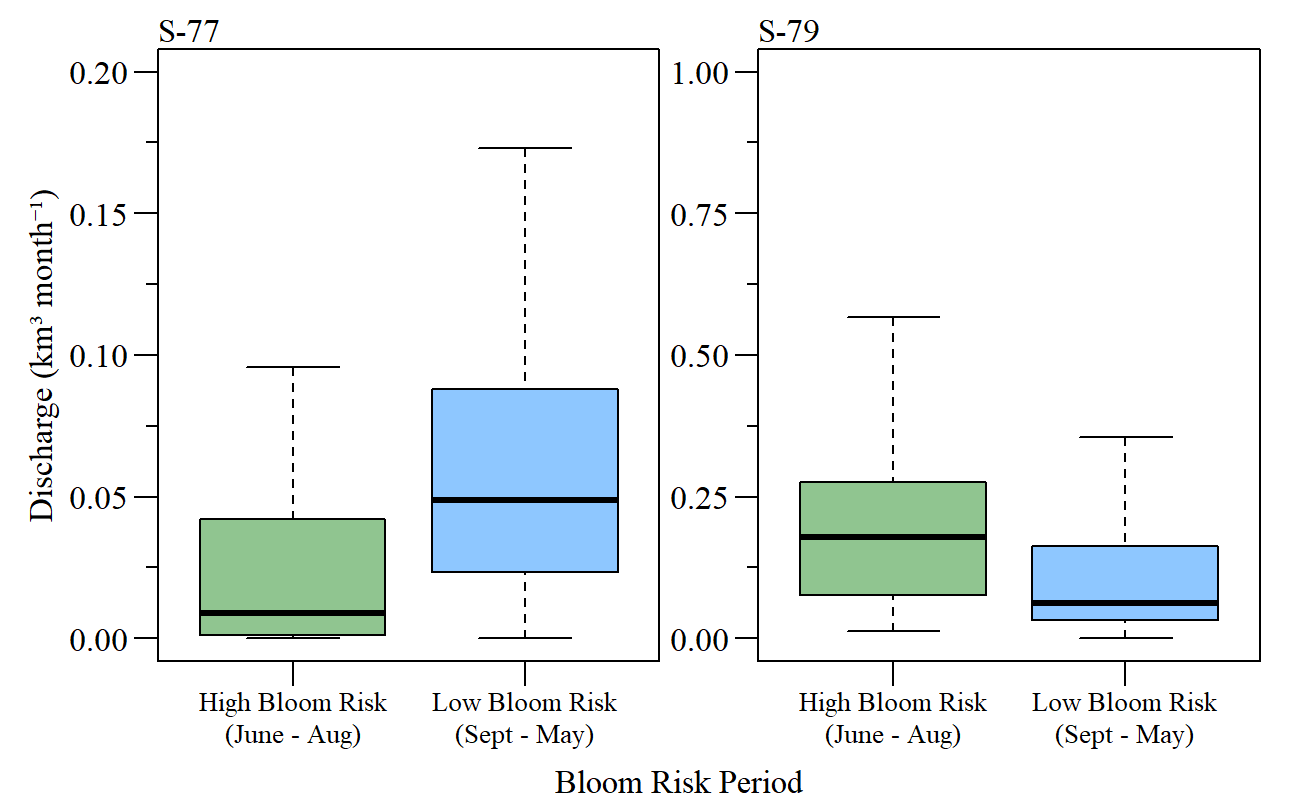
\includegraphics[width=1\linewidth]{C:/Julian_LaCie/_GitHub/LOSOM_AlgalBloom/Plots/BloomRiskPeriod} \caption{\label{fig:fig1} Comparison of monthly discharge volumes between bloom risk periods for S77 (Left) and S79 (right).}\label{fig:unnamed-chunk-3}
\end{figure}

\begin{figure}[H]
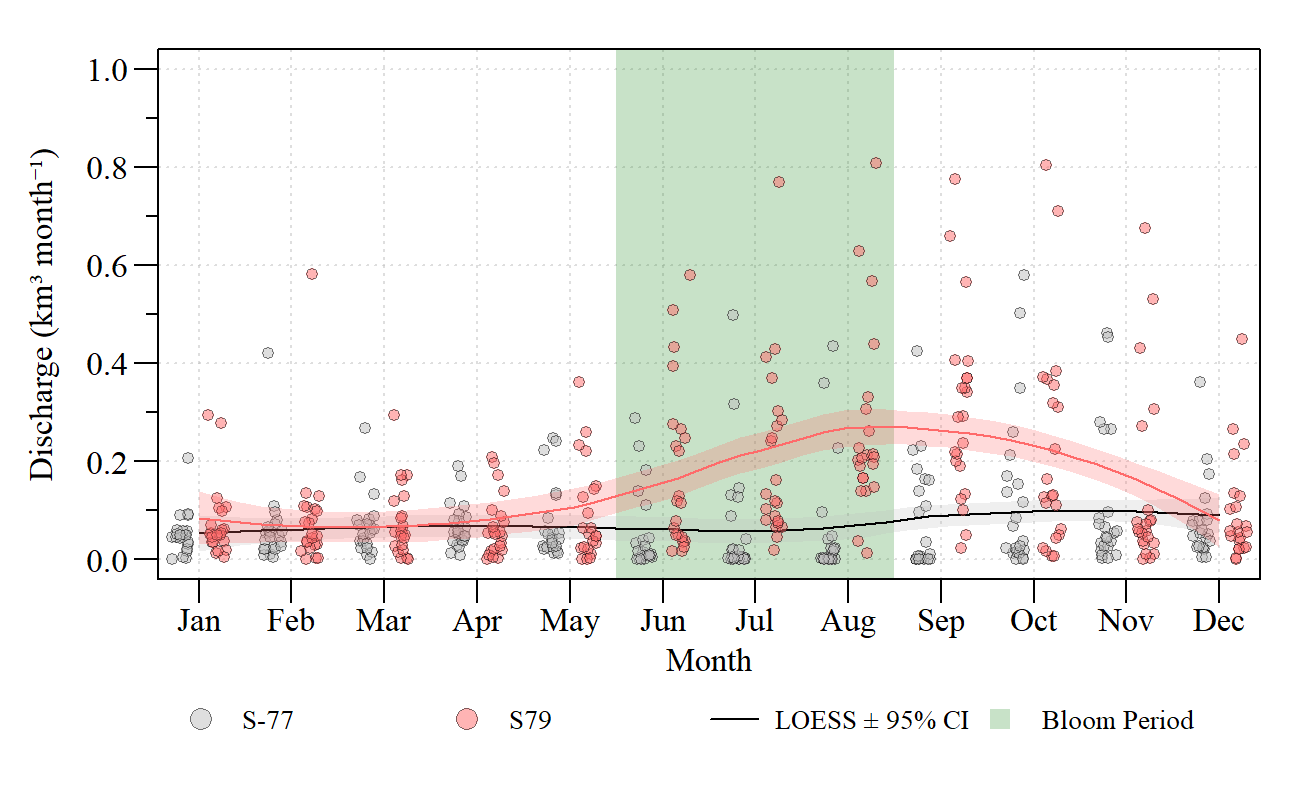
\includegraphics[width=1\linewidth]{C:/Julian_LaCie/_GitHub/LOSOM_AlgalBloom/Plots/BloomRiskPeriod_Qmonth} \caption{\label{fig:fig2} Monthly discharge volumes for S77 and S79 during the May 1999 to May 2021 period of record with locally estimated scatterplot smoothing (LOESS) trend and 95\% confidence interval.}\label{fig:unnamed-chunk-4}
\end{figure}

Monthly mean chlorophyll-a concentrations were significantly greater for
the Littoral West region relative to CRE (\(\chi^{2}\) 100, df=1,
\(\rho\)\textless0.01; Fig \ref{fig:fig3}). However, during the June to
August, high bloom period chlorophyll-a concentrations are not
significantly different between regions (\(\chi^{2}\) 0.4, df=1,
\(\rho\)=0.54; Fig \ref{fig:fig3}). However, the cross-correlation
between monthly chlorophyll-a concentration observed at CRE and that of
the Littoral West are relatively low with no correlations across the 15
month lag period (Fig \ref{fig:fig4}). To reduce the potential
variability in the data, comparison of S79 and S77 chlorophyll
concentrations were also conducted with similar results.

The logistic model to evaluate algal bloom potential at S-79 relative to
lake discharges indicated a significant decrease in log-odds ratio for
algal bloom (i.e.~chlorophyll\textgreater20 \(\mu\)g L\(^{-1}\))
relative to lake discharge (Table \ref{tab:tab2} and Fig
\ref{fig:fig5}). However, the model has a low degree of fit (McFadden's
R\(^{2}\) 0.07), therefore any algal bloom mitigation strategy developed
based on this analysis should be used with caution.

\begin{figure}[H]
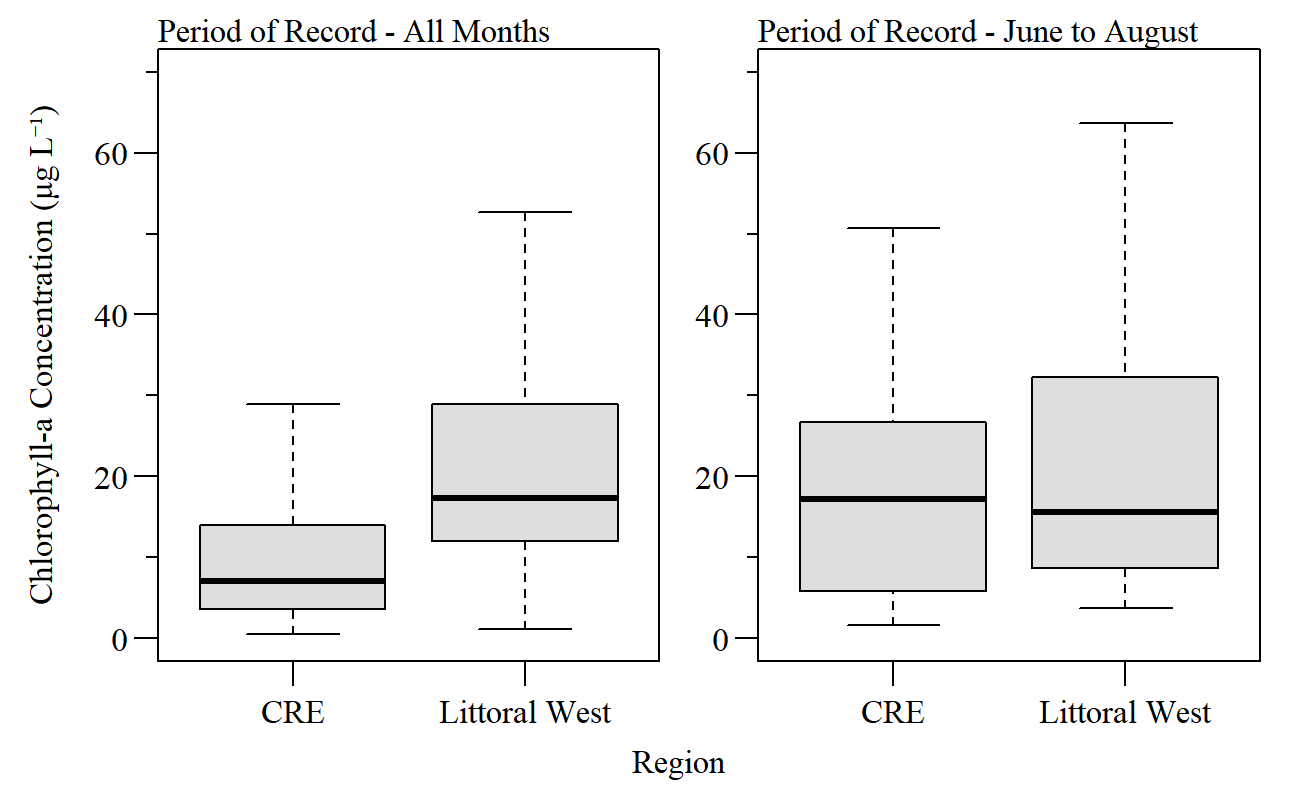
\includegraphics[width=1\linewidth]{C:/Julian_LaCie/_GitHub/LOSOM_AlgalBloom/Plots/Chl_region} \caption{\label{fig:fig3} Monthly mean chlorophyll-a concentration between regions for all months (left) and algal bloom period (right).}\label{fig:unnamed-chunk-5}
\end{figure}

\begin{figure}[H]

{\centering 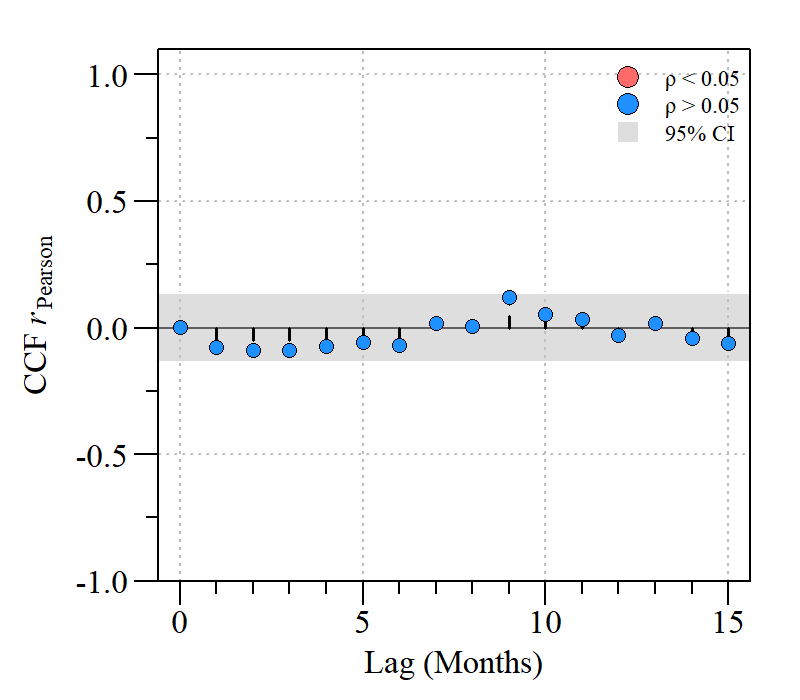
\includegraphics[width=0.7\linewidth]{C:/Julian_LaCie/_GitHub/LOSOM_AlgalBloom/Plots/Chla_CCF} 

}

\caption{\label{fig:fig4}Cross-correlation function results comparing monthly mean chlorophyll-a concentration between CRE and lagged Littoral West. }\label{fig:unnamed-chunk-6}
\end{figure}

\providecommand{\docline}[3]{\noalign{\global\setlength{\arrayrulewidth}{#1}}\arrayrulecolor[HTML]{#2}\cline{#3}}

\setlength{\tabcolsep}{2pt}

\renewcommand*{\arraystretch}{1.5}

\begin{longtable}[c]{|p{1.35in}|p{0.88in}|p{1.29in}|p{0.78in}|p{0.79in}}

\caption{\label{tab:tab2}Logistic model summary comparing algal bloom potental to lake discharges.}\\

\hhline{>{\arrayrulecolor[HTML]{666666}\global\arrayrulewidth=2pt}->{\arrayrulecolor[HTML]{666666}\global\arrayrulewidth=2pt}->{\arrayrulecolor[HTML]{666666}\global\arrayrulewidth=2pt}->{\arrayrulecolor[HTML]{666666}\global\arrayrulewidth=2pt}->{\arrayrulecolor[HTML]{666666}\global\arrayrulewidth=2pt}-}

\multicolumn{1}{!{\color[HTML]{000000}\vrule width 0pt}>{\raggedright}p{\dimexpr 1.35in+0\tabcolsep+0\arrayrulewidth}}{\fontsize{11}{11}\selectfont{\textcolor[HTML]{000000}{}}} & \multicolumn{1}{!{\color[HTML]{000000}\vrule width 0pt}>{\raggedleft}p{\dimexpr 0.88in+0\tabcolsep+0\arrayrulewidth}}{\fontsize{11}{11}\selectfont{\textcolor[HTML]{000000}{Estimate}}} & \multicolumn{1}{!{\color[HTML]{000000}\vrule width 0pt}>{\raggedleft}p{\dimexpr 1.29in+0\tabcolsep+0\arrayrulewidth}}{\fontsize{11}{11}\selectfont{\textcolor[HTML]{000000}{Standard Error}}} & \multicolumn{1}{!{\color[HTML]{000000}\vrule width 0pt}>{\raggedleft}p{\dimexpr 0.78in+0\tabcolsep+0\arrayrulewidth}}{\fontsize{11}{11}\selectfont{\textcolor[HTML]{000000}{z-value}}} & \multicolumn{1}{!{\color[HTML]{000000}\vrule width 0pt}>{\raggedleft}p{\dimexpr 0.79in+0\tabcolsep+0\arrayrulewidth}!{\color[HTML]{000000}\vrule width 0pt}}{\fontsize{11}{11}\selectfont{\textcolor[HTML]{000000}{p-value}}} \\

\noalign{\global\setlength{\arrayrulewidth}{2pt}}\arrayrulecolor[HTML]{666666}\cline{1-5}

\endfirsthead

\hhline{>{\arrayrulecolor[HTML]{666666}\global\arrayrulewidth=2pt}->{\arrayrulecolor[HTML]{666666}\global\arrayrulewidth=2pt}->{\arrayrulecolor[HTML]{666666}\global\arrayrulewidth=2pt}->{\arrayrulecolor[HTML]{666666}\global\arrayrulewidth=2pt}->{\arrayrulecolor[HTML]{666666}\global\arrayrulewidth=2pt}-}

\multicolumn{1}{!{\color[HTML]{000000}\vrule width 0pt}>{\raggedright}p{\dimexpr 1.35in+0\tabcolsep+0\arrayrulewidth}}{\fontsize{11}{11}\selectfont{\textcolor[HTML]{000000}{}}} & \multicolumn{1}{!{\color[HTML]{000000}\vrule width 0pt}>{\raggedleft}p{\dimexpr 0.88in+0\tabcolsep+0\arrayrulewidth}}{\fontsize{11}{11}\selectfont{\textcolor[HTML]{000000}{Estimate}}} & \multicolumn{1}{!{\color[HTML]{000000}\vrule width 0pt}>{\raggedleft}p{\dimexpr 1.29in+0\tabcolsep+0\arrayrulewidth}}{\fontsize{11}{11}\selectfont{\textcolor[HTML]{000000}{Standard Error}}} & \multicolumn{1}{!{\color[HTML]{000000}\vrule width 0pt}>{\raggedleft}p{\dimexpr 0.78in+0\tabcolsep+0\arrayrulewidth}}{\fontsize{11}{11}\selectfont{\textcolor[HTML]{000000}{z-value}}} & \multicolumn{1}{!{\color[HTML]{000000}\vrule width 0pt}>{\raggedleft}p{\dimexpr 0.79in+0\tabcolsep+0\arrayrulewidth}!{\color[HTML]{000000}\vrule width 0pt}}{\fontsize{11}{11}\selectfont{\textcolor[HTML]{000000}{p-value}}} \\

\noalign{\global\setlength{\arrayrulewidth}{2pt}}\arrayrulecolor[HTML]{666666}\cline{1-5}\endhead



\multicolumn{5}{!{\color[HTML]{FFFFFF}\vrule width 0pt}>{\raggedleft}p{\dimexpr 5.08in+8\tabcolsep+4\arrayrulewidth}}{\fontsize{11}{11}\selectfont{\textcolor[HTML]{000000}{\textit{(Dispersion parameter for binomial family taken to be 1)}}}} \\





\multicolumn{5}{!{\color[HTML]{FFFFFF}\vrule width 0pt}>{\raggedright}p{\dimexpr 5.08in+8\tabcolsep+4\arrayrulewidth}}{\fontsize{11}{11}\selectfont{\textcolor[HTML]{000000}{Null deviance: 183.1 on 201 degrees of freedom}}} \\





\multicolumn{5}{!{\color[HTML]{FFFFFF}\vrule width 0pt}>{\raggedright}p{\dimexpr 5.08in+8\tabcolsep+4\arrayrulewidth}}{\fontsize{11}{11}\selectfont{\textcolor[HTML]{000000}{Residual deviance: 171 on 200 degrees of freedom}}} \\





\multicolumn{5}{!{\color[HTML]{FFFFFF}\vrule width 0pt}>{\raggedright}p{\dimexpr 5.08in+8\tabcolsep+4\arrayrulewidth}}{\fontsize{11}{11}\selectfont{\textcolor[HTML]{000000}{McFadden's Pseudo R²: 0.07}}} \\

\endfoot



\multicolumn{1}{!{\color[HTML]{000000}\vrule width 0pt}>{\raggedright}p{\dimexpr 1.35in+0\tabcolsep+0\arrayrulewidth}}{\fontsize{11}{11}\selectfont{\textcolor[HTML]{000000}{(Intercept)}}} & \multicolumn{1}{!{\color[HTML]{000000}\vrule width 0pt}>{\raggedleft}p{\dimexpr 0.88in+0\tabcolsep+0\arrayrulewidth}}{\fontsize{11}{11}\selectfont{\textcolor[HTML]{000000}{-1.038}}} & \multicolumn{1}{!{\color[HTML]{000000}\vrule width 0pt}>{\raggedleft}p{\dimexpr 1.29in+0\tabcolsep+0\arrayrulewidth}}{\fontsize{11}{11}\selectfont{\textcolor[HTML]{000000}{0.246}}} & \multicolumn{1}{!{\color[HTML]{000000}\vrule width 0pt}>{\raggedleft}p{\dimexpr 0.78in+0\tabcolsep+0\arrayrulewidth}}{\fontsize{11}{11}\selectfont{\textcolor[HTML]{000000}{-4.216}}} & \multicolumn{1}{!{\color[HTML]{000000}\vrule width 0pt}>{\raggedleft}p{\dimexpr 0.79in+0\tabcolsep+0\arrayrulewidth}!{\color[HTML]{000000}\vrule width 0pt}}{\fontsize{11}{11}\selectfont{\textcolor[HTML]{000000}{0.000}}} \\





\multicolumn{1}{!{\color[HTML]{000000}\vrule width 0pt}>{\raggedright}p{\dimexpr 1.35in+0\tabcolsep+0\arrayrulewidth}}{\fontsize{11}{11}\selectfont{\textcolor[HTML]{000000}{Lake Discharge}}} & \multicolumn{1}{!{\color[HTML]{000000}\vrule width 0pt}>{\raggedleft}p{\dimexpr 0.88in+0\tabcolsep+0\arrayrulewidth}}{\fontsize{11}{11}\selectfont{\textcolor[HTML]{000000}{-12.165}}} & \multicolumn{1}{!{\color[HTML]{000000}\vrule width 0pt}>{\raggedleft}p{\dimexpr 1.29in+0\tabcolsep+0\arrayrulewidth}}{\fontsize{11}{11}\selectfont{\textcolor[HTML]{000000}{4.860}}} & \multicolumn{1}{!{\color[HTML]{000000}\vrule width 0pt}>{\raggedleft}p{\dimexpr 0.78in+0\tabcolsep+0\arrayrulewidth}}{\fontsize{11}{11}\selectfont{\textcolor[HTML]{000000}{-2.503}}} & \multicolumn{1}{!{\color[HTML]{000000}\vrule width 0pt}>{\raggedleft}p{\dimexpr 0.79in+0\tabcolsep+0\arrayrulewidth}!{\color[HTML]{000000}\vrule width 0pt}}{\fontsize{11}{11}\selectfont{\textcolor[HTML]{000000}{0.012}}} \\

\noalign{\global\setlength{\arrayrulewidth}{2pt}}\arrayrulecolor[HTML]{666666}\cline{1-5}

\end{longtable}

\begin{figure}[H]
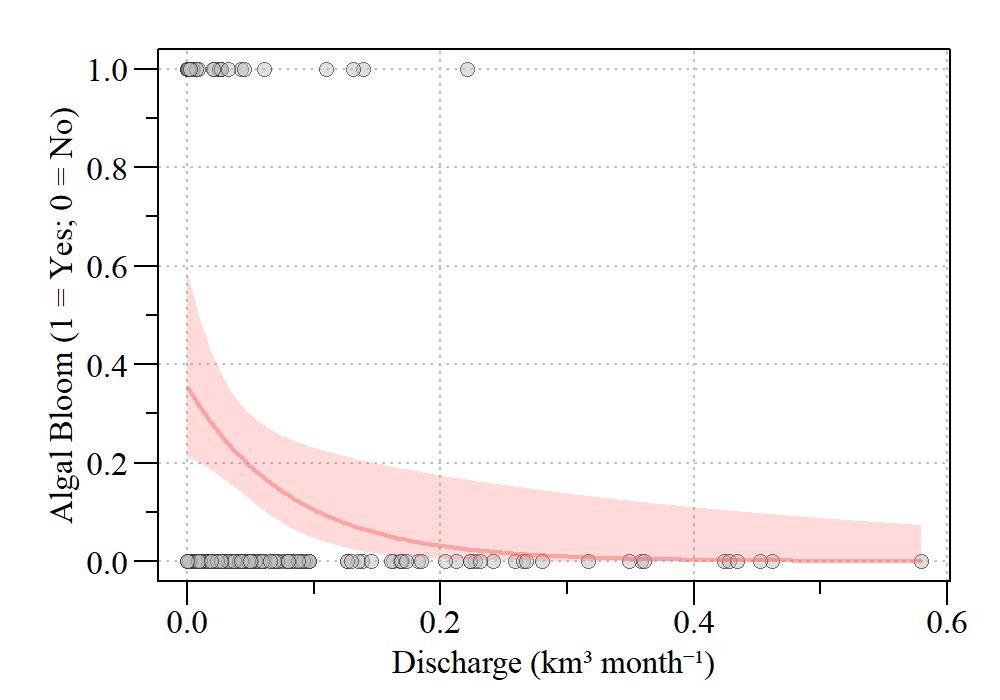
\includegraphics[width=1\linewidth]{C:/Julian_LaCie/_GitHub/LOSOM_AlgalBloom/Plots/logisticmod_CREChla} \caption{\label{fig:fig5} Algal bloom occurance at S-79 compared to lake discharges with fitted logistic model with 95\% confidence interval.}\label{fig:unnamed-chunk-9}
\end{figure}

\newpage
\appendix
\section{Reproducible R-Code}
\label{section:code}

\begin{Shaded}
\begin{Highlighting}[]
\DocumentationTok{\#\# Libraries}
\CommentTok{\#devtools::install\_github("SwampThingPaul/AnalystHelper")}
\FunctionTok{library}\NormalTok{(AnalystHelper);}

\FunctionTok{library}\NormalTok{(plyr)}
\FunctionTok{library}\NormalTok{(reshape2)}
\FunctionTok{library}\NormalTok{(zoo)}

\CommentTok{\# {-}{-}{-}{-}{-}{-}{-}{-}{-}{-}{-}{-}{-}{-}{-}{-}{-}{-}{-}{-}{-}{-}{-}{-}{-}{-}{-}{-}{-}{-}{-}{-}{-}{-}{-}{-}{-}{-}{-}{-}{-}{-}{-}{-}{-}{-}{-}{-}{-}{-}{-}{-}{-}{-}{-}{-}{-}{-}{-}{-}{-}{-}{-}{-}{-}{-}{-}{-}{-}}
\NormalTok{dates}\OtherTok{=}\FunctionTok{date.fun}\NormalTok{(}\FunctionTok{c}\NormalTok{(}\StringTok{"1999{-}05{-}01"}\NormalTok{,}\StringTok{"2021{-}04{-}30"}\NormalTok{))}

\CommentTok{\# Discharge {-}{-}{-}{-}{-}{-}{-}{-}{-}{-}{-}{-}{-}{-}{-}{-}{-}{-}{-}{-}{-}{-}{-}{-}{-}{-}{-}{-}{-}{-}{-}{-}{-}{-}{-}{-}{-}{-}{-}{-}{-}{-}{-}{-}{-}{-}{-}{-}{-}{-}{-}{-}{-}{-}{-}{-}{-}{-}{-}}
\NormalTok{q.dbkeys}\OtherTok{=}\FunctionTok{data.frame}\NormalTok{(}\AttributeTok{SITE=}\FunctionTok{c}\NormalTok{(}\StringTok{"S79"}\NormalTok{,}\StringTok{"S78"}\NormalTok{,}\StringTok{"S77"}\NormalTok{),}
                    \AttributeTok{DBKEY=}\FunctionTok{c}\NormalTok{(}\StringTok{"00865"}\NormalTok{,}\StringTok{"DJ236"}\NormalTok{,}\StringTok{"15635"}\NormalTok{))}
\NormalTok{q.cre.dat}\OtherTok{=}\FunctionTok{data.frame}\NormalTok{()}
\ControlFlowTok{for}\NormalTok{(i }\ControlFlowTok{in} \DecValTok{1}\SpecialCharTok{:}\FunctionTok{nrow}\NormalTok{(q.dbkeys))\{}
\NormalTok{  tmp}\OtherTok{=}\FunctionTok{DBHYDRO\_daily}\NormalTok{(dates[}\DecValTok{1}\NormalTok{],dates[}\DecValTok{2}\NormalTok{],q.dbkeys}\SpecialCharTok{$}\NormalTok{DBKEY[i])}
\NormalTok{  tmp}\SpecialCharTok{$}\NormalTok{DBKEY}\OtherTok{=}\FunctionTok{as.character}\NormalTok{(q.dbkeys}\SpecialCharTok{$}\NormalTok{DBKEY[i])}
\NormalTok{  q.cre.dat}\OtherTok{=}\FunctionTok{rbind}\NormalTok{(q.cre.dat,tmp)}
  \FunctionTok{print}\NormalTok{(i)}
\NormalTok{\}}
\NormalTok{q.cre.dat}\OtherTok{=}\FunctionTok{merge}\NormalTok{(q.cre.dat,q.dbkeys,}\StringTok{"DBKEY"}\NormalTok{)}
\NormalTok{q.cre.dat}\SpecialCharTok{$}\NormalTok{Date.EST}\OtherTok{=}\FunctionTok{date.fun}\NormalTok{(q.cre.dat}\SpecialCharTok{$}\NormalTok{Date)}

\NormalTok{q.cre.dat.xtab}\OtherTok{=}\FunctionTok{dcast}\NormalTok{(q.cre.dat,Date.EST}\SpecialCharTok{\textasciitilde{}}\NormalTok{SITE,}
                     \AttributeTok{value.var=}\StringTok{"Data.Value"}\NormalTok{,mean)}
\NormalTok{q.cre.dat.xtab}\SpecialCharTok{$}\NormalTok{month}\OtherTok{=}\FunctionTok{as.numeric}\NormalTok{(}\FunctionTok{format}\NormalTok{(q.cre.dat.xtab}\SpecialCharTok{$}\NormalTok{Date,}\StringTok{"\%m"}\NormalTok{))}
\NormalTok{q.cre.dat.xtab}\SpecialCharTok{$}\NormalTok{CY}\OtherTok{=}\FunctionTok{as.numeric}\NormalTok{(}\FunctionTok{format}\NormalTok{(q.cre.dat.xtab}\SpecialCharTok{$}\NormalTok{Date,}\StringTok{"\%Y"}\NormalTok{))}
\NormalTok{q.cre.dat.xtab}\SpecialCharTok{$}\NormalTok{monCY}\OtherTok{=}\FunctionTok{with}\NormalTok{(q.cre.dat.xtab,}
                          \FunctionTok{date.fun}\NormalTok{(}\FunctionTok{paste}\NormalTok{(CY,month,}\StringTok{"01"}\NormalTok{,}\AttributeTok{sep=}\StringTok{"{-}"}\NormalTok{)))}
\NormalTok{q.cre.dat.xtab}\SpecialCharTok{$}\NormalTok{WY}\OtherTok{=}\FunctionTok{WY}\NormalTok{(q.cre.dat.xtab}\SpecialCharTok{$}\NormalTok{Date.EST)}

\CommentTok{\#Positive discharge only}
\NormalTok{q.cre.dat.xtab}\SpecialCharTok{$}\NormalTok{S77}\OtherTok{=}\FunctionTok{with}\NormalTok{(q.cre.dat.xtab,}\FunctionTok{ifelse}\NormalTok{(S77}\SpecialCharTok{\textless{}}\DecValTok{0}\NormalTok{,}\DecValTok{0}\NormalTok{,S77))}
\NormalTok{q.cre.dat.xtab}\SpecialCharTok{$}\NormalTok{S79}\OtherTok{=}\FunctionTok{with}\NormalTok{(q.cre.dat.xtab,}\FunctionTok{ifelse}\NormalTok{(S79}\SpecialCharTok{\textless{}}\DecValTok{0}\NormalTok{,}\DecValTok{0}\NormalTok{,S79))}
\NormalTok{q.cre.dat.xtab}\SpecialCharTok{$}\NormalTok{C43}\OtherTok{=}\FunctionTok{with}\NormalTok{(q.cre.dat.xtab,}\FunctionTok{ifelse}\NormalTok{(S79}\SpecialCharTok{\textless{}}\NormalTok{S77,}\DecValTok{0}\NormalTok{,S79}\SpecialCharTok{{-}}\NormalTok{S77))}
\NormalTok{q.cre.dat.xtab}\SpecialCharTok{$}\NormalTok{Lake}\OtherTok{=}\FunctionTok{with}\NormalTok{(q.cre.dat.xtab,}\FunctionTok{ifelse}\NormalTok{(S77}\SpecialCharTok{\textless{}}\NormalTok{S79,}\DecValTok{0}\NormalTok{,S77}\SpecialCharTok{{-}}\NormalTok{S79))}

\NormalTok{q.cre.dat.xtab.mon}\OtherTok{=}\FunctionTok{ddply}\NormalTok{(q.cre.dat.xtab,}\FunctionTok{c}\NormalTok{(}\StringTok{"monCY"}\NormalTok{,}\StringTok{"month"}\NormalTok{,}\StringTok{\textquotesingle{}CY\textquotesingle{}}\NormalTok{),}
\NormalTok{                         summarise,}
                         \AttributeTok{S77=}\FunctionTok{sum}\NormalTok{(}\FunctionTok{cfs.to.km3d}\NormalTok{(S77),}\AttributeTok{na.rm=}\NormalTok{T),}
                         \AttributeTok{S79=}\FunctionTok{sum}\NormalTok{(}\FunctionTok{cfs.to.km3d}\NormalTok{(S79),}\AttributeTok{na.rm=}\NormalTok{T))}
\NormalTok{q.cre.dat.xtab.mon}\SpecialCharTok{$}\NormalTok{C43}\OtherTok{=}\FunctionTok{with}\NormalTok{(q.cre.dat.xtab.mon,}
                            \FunctionTok{ifelse}\NormalTok{(S79}\SpecialCharTok{\textless{}}\NormalTok{S77,}\DecValTok{0}\NormalTok{,S79}\SpecialCharTok{{-}}\NormalTok{S77))}
\NormalTok{q.cre.dat.xtab.mon}\SpecialCharTok{$}\NormalTok{Lake}\OtherTok{=}\FunctionTok{with}\NormalTok{(q.cre.dat.xtab.mon,}
                             \FunctionTok{ifelse}\NormalTok{(S77}\SpecialCharTok{\textgreater{}}\NormalTok{S79,S79,S77))}
\NormalTok{q.cre.dat.xtab.mon}\SpecialCharTok{$}\NormalTok{Period}\OtherTok{=}\FunctionTok{with}\NormalTok{(q.cre.dat.xtab.mon,}
                               \FunctionTok{ifelse}\NormalTok{(month}\SpecialCharTok{\%in\%}\FunctionTok{c}\NormalTok{(}\DecValTok{6}\SpecialCharTok{:}\DecValTok{8}\NormalTok{),}
                                      \StringTok{"Bloom"}\NormalTok{,}\StringTok{"Non{-}Bloom"}\NormalTok{))}

\DocumentationTok{\#\# Comparison of monthly discharge }
\DocumentationTok{\#\# between bloom/non{-}bloom periods}

\FunctionTok{boxplot}\NormalTok{(S77}\SpecialCharTok{\textasciitilde{}}\NormalTok{Period,q.cre.dat.xtab.mon)}
\FunctionTok{kruskal.test}\NormalTok{(S77}\SpecialCharTok{\textasciitilde{}}\NormalTok{Period,q.cre.dat.xtab.mon)}

\FunctionTok{boxplot}\NormalTok{(S79}\SpecialCharTok{\textasciitilde{}}\NormalTok{Period,q.cre.dat.xtab.mon)}
\FunctionTok{kruskal.test}\NormalTok{(S79}\SpecialCharTok{\textasciitilde{}}\NormalTok{Period,q.cre.dat.xtab.mon)}

\CommentTok{\# WQ Data {-}{-}{-}{-}{-}{-}{-}{-}{-}{-}{-}{-}{-}{-}{-}{-}{-}{-}{-}{-}{-}{-}{-}{-}{-}{-}{-}{-}{-}{-}{-}{-}{-}{-}{-}{-}{-}{-}{-}{-}{-}{-}{-}{-}{-}{-}{-}{-}{-}{-}{-}{-}{-}{-}{-}{-}{-}{-}{-}{-}{-}}

\NormalTok{params}\OtherTok{=}\FunctionTok{data.frame}\NormalTok{(}\AttributeTok{Test.Number=}\FunctionTok{c}\NormalTok{(}\DecValTok{61}\NormalTok{,}\DecValTok{179}\NormalTok{),}
                  \AttributeTok{param=}\FunctionTok{c}\NormalTok{(}\StringTok{"Chla"}\NormalTok{,}\StringTok{"Chla"}\NormalTok{))}

\NormalTok{wq.sites}\OtherTok{=}\FunctionTok{data.frame}\NormalTok{(}\AttributeTok{Station.ID=}
                      \FunctionTok{c}\NormalTok{(}\StringTok{"S79"}\NormalTok{,}\StringTok{"CES01"}\NormalTok{,}\StringTok{"S77"}\NormalTok{,}
                        \StringTok{"PALMOUT"}\NormalTok{,}\StringTok{"PLN2OUT"}\NormalTok{,}\StringTok{"TREEOUT"}\NormalTok{),}
                    \AttributeTok{Region=}\FunctionTok{c}\NormalTok{(}\FunctionTok{rep}\NormalTok{(}\StringTok{"CRE"}\NormalTok{,}\DecValTok{2}\NormalTok{),}\FunctionTok{rep}\NormalTok{(}\StringTok{"LitWest"}\NormalTok{,}\DecValTok{4}\NormalTok{)))}

\NormalTok{wq.dat}\OtherTok{=}\FunctionTok{DBHYDRO\_WQ}\NormalTok{(dates[}\DecValTok{1}\NormalTok{],dates[}\DecValTok{2}\NormalTok{],}
\NormalTok{                  wq.sites}\SpecialCharTok{$}\NormalTok{Station.ID,params}\SpecialCharTok{$}\NormalTok{Test.Number)}
\NormalTok{wq.dat}\OtherTok{=}\FunctionTok{merge}\NormalTok{(wq.dat,params,}\StringTok{"Test.Number"}\NormalTok{)}
\FunctionTok{unique}\NormalTok{(wq.dat}\SpecialCharTok{$}\NormalTok{Collection.Method)}
\NormalTok{wq.dat}\OtherTok{=}\FunctionTok{subset}\NormalTok{(wq.dat,Collection.Method}\SpecialCharTok{==}\StringTok{"G"}\NormalTok{)}

\NormalTok{wq.dat.xtab}\OtherTok{=}\FunctionTok{dcast}\NormalTok{(wq.dat,Station.ID}\SpecialCharTok{+}\NormalTok{Date.EST}\SpecialCharTok{\textasciitilde{}}\NormalTok{param,}
                  \AttributeTok{value.var=}\StringTok{"HalfMDL"}\NormalTok{,mean)}
\NormalTok{wq.dat.xtab}\SpecialCharTok{$}\NormalTok{WY}\OtherTok{=}\FunctionTok{WY}\NormalTok{(wq.dat.xtab}\SpecialCharTok{$}\NormalTok{Date.EST)}
\NormalTok{wq.dat.xtab}\SpecialCharTok{$}\NormalTok{month}\OtherTok{=}\FunctionTok{as.numeric}\NormalTok{(}\FunctionTok{format}\NormalTok{(wq.dat.xtab}\SpecialCharTok{$}\NormalTok{Date.EST,}\StringTok{"\%m"}\NormalTok{))}
\NormalTok{wq.dat.xtab}\SpecialCharTok{$}\NormalTok{CY}\OtherTok{=}\FunctionTok{as.numeric}\NormalTok{(}\FunctionTok{format}\NormalTok{(wq.dat.xtab}\SpecialCharTok{$}\NormalTok{Date.EST,}\StringTok{"\%Y"}\NormalTok{))}
\NormalTok{wq.dat.xtab}\SpecialCharTok{$}\NormalTok{monCY}\OtherTok{=}\FunctionTok{with}\NormalTok{(wq.dat.xtab,}
                       \FunctionTok{date.fun}\NormalTok{(}\FunctionTok{paste}\NormalTok{(CY,month,}\StringTok{"01"}\NormalTok{,}\AttributeTok{sep=}\StringTok{"{-}"}\NormalTok{)))}
\NormalTok{wq.dat.xtab}\OtherTok{=}\FunctionTok{merge}\NormalTok{(wq.dat.xtab,wq.sites,}\StringTok{"Station.ID"}\NormalTok{)}

\DocumentationTok{\#\# Regional Comparison}
\NormalTok{Chla.region}\OtherTok{=}\FunctionTok{ddply}\NormalTok{(wq.dat.xtab,}\FunctionTok{c}\NormalTok{(}\StringTok{"monCY"}\NormalTok{,}\StringTok{"month"}\NormalTok{,}\StringTok{"Region"}\NormalTok{),}
\NormalTok{                  summarise,}\AttributeTok{mean.val=}\FunctionTok{mean}\NormalTok{(Chla,}\AttributeTok{na.rm=}\NormalTok{T))}
\NormalTok{Chla.region}\SpecialCharTok{$}\NormalTok{bloom}\OtherTok{=}\FunctionTok{ifelse}\NormalTok{(Chla.region}\SpecialCharTok{$}\NormalTok{mean.val}\SpecialCharTok{\textgreater{}}\DecValTok{20}\NormalTok{,}\DecValTok{1}\NormalTok{,}\DecValTok{0}\NormalTok{)}

\FunctionTok{kruskal.test}\NormalTok{(mean.val}\SpecialCharTok{\textasciitilde{}}\NormalTok{Region,Chla.region)}
\FunctionTok{kruskal.test}\NormalTok{(mean.val}\SpecialCharTok{\textasciitilde{}}\NormalTok{Region,}\FunctionTok{subset}\NormalTok{(Chla.region,month}\SpecialCharTok{\%in\%}\FunctionTok{c}\NormalTok{(}\DecValTok{6}\SpecialCharTok{:}\DecValTok{8}\NormalTok{)))}
\FunctionTok{plot}\NormalTok{(mean.val}\SpecialCharTok{\textasciitilde{}}\NormalTok{month,}\FunctionTok{subset}\NormalTok{(Chla.region,Region}\SpecialCharTok{==}\StringTok{"CRE"}\NormalTok{))}
\FunctionTok{plot}\NormalTok{(mean.val}\SpecialCharTok{\textasciitilde{}}\NormalTok{month,}\FunctionTok{subset}\NormalTok{(Chla.region,Region}\SpecialCharTok{==}\StringTok{"LitWest"}\NormalTok{))}

\DocumentationTok{\#\# Cross Correlation}
\NormalTok{Chla.region.xtab}\OtherTok{=}\FunctionTok{dcast}\NormalTok{(wq.dat.xtab,monCY}\SpecialCharTok{\textasciitilde{}}\NormalTok{Region,}
                       \AttributeTok{value.var =} \StringTok{"Chla"}\NormalTok{,}
                       \AttributeTok{fun.aggregate=}\ControlFlowTok{function}\NormalTok{(x) }\FunctionTok{mean}\NormalTok{(x,}\AttributeTok{na.rm=}\NormalTok{T))}
\FunctionTok{plot}\NormalTok{(CRE}\SpecialCharTok{\textasciitilde{}}\NormalTok{LitWest,Chla.region.xtab)}

\NormalTok{Chla.region.xtab}\OtherTok{=}\FunctionTok{merge}\NormalTok{(Chla.region.xtab,q.cre.dat.xtab.mon,}\StringTok{"monCY"}\NormalTok{)}

\FunctionTok{layout}\NormalTok{(}\FunctionTok{matrix}\NormalTok{(}\DecValTok{1}\SpecialCharTok{:}\DecValTok{4}\NormalTok{,}\DecValTok{1}\NormalTok{,}\DecValTok{4}\NormalTok{,}\AttributeTok{byrow=}\NormalTok{T))}
\ControlFlowTok{for}\NormalTok{(h }\ControlFlowTok{in} \DecValTok{0}\SpecialCharTok{:}\DecValTok{3}\NormalTok{)\{}
\NormalTok{  tmp.dat}\OtherTok{=}\FunctionTok{data.frame}\NormalTok{(}\AttributeTok{CRE.chla=}\FunctionTok{lag}\NormalTok{(}\FunctionTok{as.zoo}\NormalTok{(Chla.region.xtab}\SpecialCharTok{$}\NormalTok{CRE),}
                                  \DecValTok{0}\NormalTok{,}\AttributeTok{na.pad=}\NormalTok{T),}
                     \AttributeTok{Lake.chla=}\FunctionTok{lag}\NormalTok{(}\FunctionTok{as.zoo}\NormalTok{(Chla.region.xtab}\SpecialCharTok{$}\NormalTok{LitWest),}
                                   \SpecialCharTok{{-}}\NormalTok{h,}\AttributeTok{na.pad=}\NormalTok{T),}
                     \AttributeTok{Lake=}\NormalTok{Chla.region.xtab}\SpecialCharTok{$}\NormalTok{Lake)}
  \FunctionTok{plot}\NormalTok{(CRE.chla}\SpecialCharTok{\textasciitilde{}}\NormalTok{Lake.chla,tmp.dat,}\AttributeTok{pch=}\DecValTok{21}\NormalTok{,}\StringTok{"grey"}\NormalTok{)}
\NormalTok{\}}

\CommentTok{\# ccf function in R}
\FunctionTok{with}\NormalTok{(}\FunctionTok{subset}\NormalTok{(Chla.region.xtab,}\FunctionTok{is.na}\NormalTok{(CRE)}\SpecialCharTok{==}\NormalTok{F}\SpecialCharTok{\&}\FunctionTok{is.na}\NormalTok{(LitWest)}\SpecialCharTok{==}\NormalTok{F),}
     \FunctionTok{ccf}\NormalTok{(CRE,LitWest,}\AttributeTok{type=}\StringTok{"correlation"}\NormalTok{))}

\NormalTok{ccf.chla.rslt}\OtherTok{=}\FunctionTok{data.frame}\NormalTok{()}
\ControlFlowTok{for}\NormalTok{(h }\ControlFlowTok{in} \DecValTok{0}\SpecialCharTok{:}\DecValTok{15}\NormalTok{)\{}
\NormalTok{  lagged}\OtherTok{=}\FunctionTok{lag}\NormalTok{(}\FunctionTok{as.zoo}\NormalTok{(Chla.region.xtab}\SpecialCharTok{$}\NormalTok{LitWest),}\SpecialCharTok{{-}}\NormalTok{h,}\AttributeTok{na.pad=}\NormalTok{T)}
\NormalTok{  tmp.dat}\OtherTok{=}\FunctionTok{as.zoo}\NormalTok{(Chla.region.xtab}\SpecialCharTok{$}\NormalTok{CRE)}
\NormalTok{  stat}\OtherTok{=}\FunctionTok{with}\NormalTok{(}\FunctionTok{data.frame}\NormalTok{(}\AttributeTok{lag=}\NormalTok{lagged,}\AttributeTok{dat=}\NormalTok{tmp.dat),}
            \FunctionTok{cor.test}\NormalTok{(lag,dat,}\AttributeTok{method=}\StringTok{"pearson"}\NormalTok{))}
\NormalTok{  ccf.chla.rslt}\OtherTok{=}\FunctionTok{rbind}\NormalTok{(ccf.chla.rslt,}
                      \FunctionTok{data.frame}\NormalTok{(}\AttributeTok{lag=}\NormalTok{h,}
                                 \AttributeTok{estimate=}\FunctionTok{as.numeric}\NormalTok{(stat}\SpecialCharTok{$}\NormalTok{estimate),}
                                 \AttributeTok{pval=}\NormalTok{stat}\SpecialCharTok{$}\NormalTok{p.value))}
\NormalTok{\}}
\NormalTok{ccf.chla.rslt}


\DocumentationTok{\#\# Logistic Regression}
\CommentTok{\# data prep}
\NormalTok{bloom.region.xtab}\OtherTok{=}\FunctionTok{dcast}\NormalTok{(Chla.region,monCY}\SpecialCharTok{\textasciitilde{}}\NormalTok{Region,}
                        \AttributeTok{value.var =} \StringTok{"bloom"}\NormalTok{,}
                        \AttributeTok{fun.aggregate=}\ControlFlowTok{function}\NormalTok{(x) }\FunctionTok{mean}\NormalTok{(x,}\AttributeTok{na.rm=}\NormalTok{T))}
\NormalTok{bloom.region.xtab}\SpecialCharTok{$}\NormalTok{bothbloom}\OtherTok{=}\FunctionTok{with}\NormalTok{(bloom.region.xtab,}
                                 \FunctionTok{ifelse}\NormalTok{(CRE}\SpecialCharTok{==}\DecValTok{1}\SpecialCharTok{\&}\NormalTok{LitWest}\SpecialCharTok{==}\DecValTok{1}\NormalTok{,}\DecValTok{1}\NormalTok{,}\DecValTok{0}\NormalTok{))}
\NormalTok{bloom.region.xtab2}\OtherTok{=}\FunctionTok{merge}\NormalTok{(bloom.region.xtab,}
\NormalTok{                         q.cre.dat.xtab.mon,}
                         \StringTok{"monCY"}\NormalTok{)}

\CommentTok{\# Data Explore}
\FunctionTok{plot}\NormalTok{(CRE}\SpecialCharTok{\textasciitilde{}}\NormalTok{Lake,bloom.region.xtab2)}
\FunctionTok{plot}\NormalTok{(CRE}\SpecialCharTok{\textasciitilde{}}\NormalTok{S77,bloom.region.xtab2)}
\FunctionTok{plot}\NormalTok{(bothbloom}\SpecialCharTok{\textasciitilde{}}\NormalTok{Lake,bloom.region.xtab2)}
\FunctionTok{plot}\NormalTok{(bothbloom}\SpecialCharTok{\textasciitilde{}}\NormalTok{S77,bloom.region.xtab2)}

\NormalTok{mod}\OtherTok{=}\FunctionTok{glm}\NormalTok{(CRE}\SpecialCharTok{\textasciitilde{}}\NormalTok{Lake,bloom.region.xtab2,}\AttributeTok{family=}\StringTok{"binomial"}\NormalTok{)}
\FunctionTok{summary}\NormalTok{(mod)}
\FunctionTok{confint}\NormalTok{(mod)}

\CommentTok{\# diagonistics}
\FunctionTok{plot}\NormalTok{(}\DecValTok{1}\SpecialCharTok{:}\FunctionTok{length}\NormalTok{(}\FunctionTok{rstandard}\NormalTok{(mod)),}\FunctionTok{rstandard}\NormalTok{(mod))}
\FunctionTok{plot}\NormalTok{(mod,}\AttributeTok{which=}\DecValTok{4}\NormalTok{,}\AttributeTok{id.n=}\DecValTok{5}\NormalTok{);}\CommentTok{\#identify the top five largest values}

\CommentTok{\# McFadden\textquotesingle{}s r2}
\NormalTok{glm.null.loglike}\OtherTok{=}\FunctionTok{logLik}\NormalTok{(}\FunctionTok{glm}\NormalTok{(CRE}\SpecialCharTok{\textasciitilde{}}\DecValTok{1}\NormalTok{,}
\NormalTok{                            bloom.region.xtab2,}
                            \AttributeTok{family=}\StringTok{"binomial"}\NormalTok{))[}\DecValTok{1}\NormalTok{]}
\NormalTok{mcR2}\OtherTok{=}\DecValTok{1}\SpecialCharTok{{-}}\FunctionTok{logLik}\NormalTok{(mod)[}\DecValTok{1}\NormalTok{]}\SpecialCharTok{/}\NormalTok{glm.null.loglike}
\NormalTok{mcR2}

\CommentTok{\#classification rate}
\FunctionTok{prop.table}\NormalTok{(}\FunctionTok{table}\NormalTok{(bloom.region.xtab2}\SpecialCharTok{$}\NormalTok{CRE,}
                 \FunctionTok{predict}\NormalTok{(mod,}
                         \FunctionTok{data.frame}\NormalTok{(}\AttributeTok{Lake=}\NormalTok{bloom.region.xtab2}\SpecialCharTok{$}\NormalTok{Lake),}
                         \AttributeTok{type=}\StringTok{"response"}\NormalTok{)}\SpecialCharTok{\textgreater{}}\FloatTok{0.5}\NormalTok{))}
\end{Highlighting}
\end{Shaded}

\newpage
\section{Sample Map}

\begin{figure}[H]

{\centering 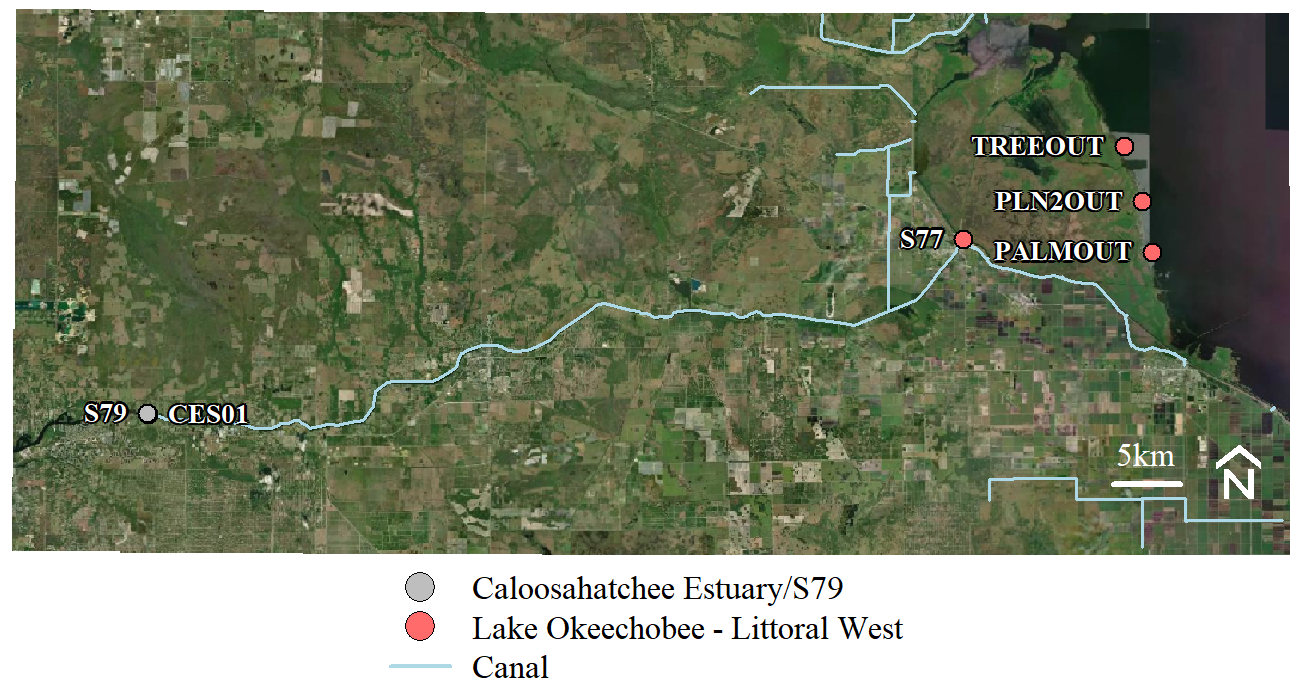
\includegraphics[width=1.1\linewidth]{C:/Julian_LaCie/_GitHub/LOSOM_AlgalBloom/Plots/MonitoringMap} 

}

\caption{\label{fig:map}Map of monitoring locations presented in Table \ref{tab:tab1}.}\label{fig:unnamed-chunk-11}
\end{figure}

\newpage

\bibliographystyle{tfcad}
\bibliography{refs.bib}




\end{document}